%%%%%%%%%%%%%%%%%%%%%%%%%%%%%%%%%%%%%%%%%
% LaTeX Template
% http://www.LaTeXTemplates.com
%
% Original author:
% Linux and Unix Users Group at Virginia Tech Wiki 
% (https://vtluug.org/wiki/Example_LaTeX_chem_lab_report)
%
% License:
% CC BY-NC-SA 3.0 (http://creativecommons.org/licenses/by-nc-sa/3.0/)
%
%%%%%%%%%%%%%%%%%%%%%%%%%%%%%%%%%%%%%%%%%

%----------------------------------------------------------------------------------------
%	PACKAGES AND DOCUMENT CONFIGURATIONS
%----------------------------------------------------------------------------------------

\documentclass[11pt]{article}
\usepackage{geometry} % Pour passer au format A4
\geometry{hmargin=1cm, vmargin=1cm} % 

\usepackage{graphicx} % Required for including pictures
\usepackage{float} % 

%Français
\usepackage[T1]{fontenc} 
\usepackage[english,francais]{babel}
\usepackage[utf8]{inputenc}
\usepackage{eurosym}
\usepackage{lmodern}
\usepackage{url}
\usepackage{multicol}

%Maths
\usepackage{amsmath,amsfonts,amssymb,amsthm}
%\usepackage[linesnumbered, ruled, vlined]{algorithm2e}
%\SetAlFnt{\small\sffamily}

%Autres
\linespread{1} % Line spacing
\setlength\parindent{0pt} % Removes all indentation from paragraphs

\renewcommand{\labelenumi}{\alph{enumi}.} % 
\pagestyle{empty}
%----------------------------------------------------------------------------------------
%	DOCUMENT INFORMATION
%----------------------------------------------------------------------------------------
\begin{document}

%\maketitle % Insert the title, author and date

\begin{minipage}[t]{\textwidth}
  \raggedright
      {\bfseries Série : \textbf{B}}\\
      {\bfseries $5^{e}1$}\\[.35ex]
      \vspace*{-1cm}
      \raggedleft
          {\bfseries Angles relatifs}\\[.35ex]
          {\bfseries 19 Mai 2014}\\[.35ex]
\end{minipage}\\[1em]

\begin{center}
  \textsf{The secret to building large apps is never build large apps. Break your applications into small pieces. Then, assemble those testable, bite-sized pieces into your big application.}
  \texttt{Justin Meyer, author JavaScript MVC}\\
\end{center}

\setlength{\columnseprule}{1pt}
\begin{multicols}{2}
  \subsection*{1 - $Alors$ ?}

  Les droites (DF) et (BC) sont-elles parallèles ? \newline \textbf{JUSTIFIER !}] 
    \begin{figure}[H]
      \centering
      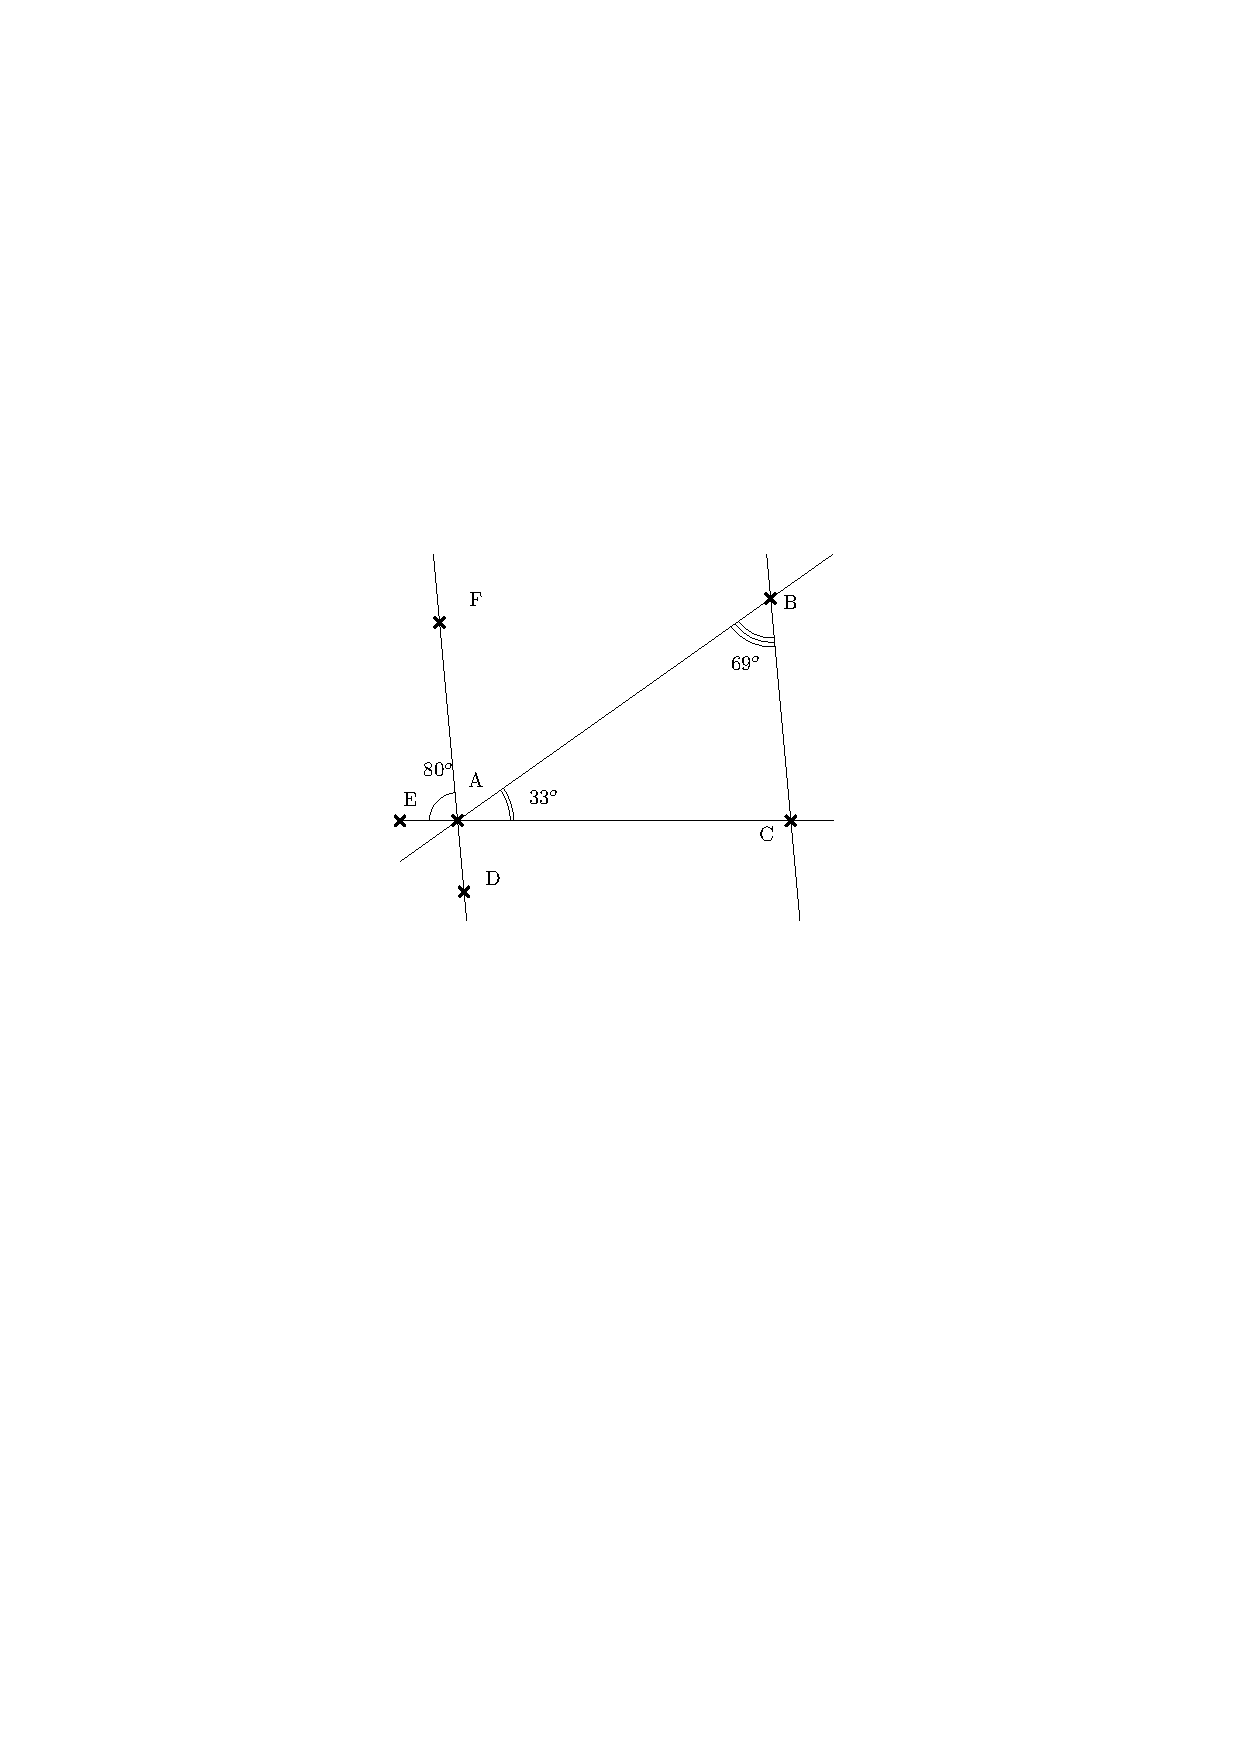
\includegraphics[width=0.8\linewidth]{sources/ie/44-2.pdf}
    \end{figure}

    \subsection*{2 - $Alors^{2}$ ?}
    Soit MNOP un rectangle. Ses deux diagonales se coupent en A.
    \textbf{En justifiant autant que possible.}
    \begin{enumerate}
    \item Tracer à main levée le rectangle et ses diagonales.
    \item Citer un angle complémentaire à $\widehat{MNA}$.
    \item Citer un angle supplémentaire à $\widehat{MAN}$.
    \item Citer deux angles opposés par le sommet. 
    \item Citer un angle alterne-interne à  $\widehat{MPA}$.
    \item Citer un angle alterne-interne à  $\widehat{APO}$.
    \item Soit $\widehat{MNA} = 36^{o}$.\\ Écrire sur la figure \textbf{toutes} les mesures d'angles possibles. 
    \end{enumerate}
\end{multicols}


\end{document}
